% #############################################################################
% This is Appendix B
% !TEX root = ../main.tex
% #############################################################################
\chapter{Some useful insights to the Method of Fundamental Solutions}
\label{chapter:appendixB}

This appendix presents some useful results and techniques which can be used to increase the accuracy of the Method of Fundamental Solutions. Firstly, we present the behavior of the Laplace equation's solutions in polar coordinates near a corner's tip. Such considerations were the basis for the results presented in \ref{numerical_transmission_simulations}. Then, the Subspace Angle Technique is also presented, which was used in \ref{dirac_equation_simulations} to tackle the ill-conditioning of the \ac{MFS} for the Dirac equation with infinite mass boundary conditions.

\section{Behavior of the Laplace equation's solutions near a corner.}\label{appendixB_corners}


In this section, the behavior of the Laplace equation's solutions near a corner is summarized for different boundary conditions. For more details, we point the reader to \cite{li2000singularities}.

\begin{itemize}
    \item For Dirichlet-Dirichlet boundary conditions given by \(u(r, 0) = A, u(r, \Theta) = B\), then \(\alpha_k = \frac{k \pi}{\Theta}\) and
    \[
        u(r, \theta) = A (B-A)\frac{\theta}{\Theta} + \sum_{k=0}^{\infty}\alpha_k r^{\alpha_k}\sin(\alpha_k \theta);
    \]
    \item For Dirichlet-Neumann boundary conditions given by \(u(r, 0) = A, \partial_n u(r, \Theta) = B\), then \(\alpha_k = \frac{\left(k+\frac{1}{2}\right) \pi}{\Theta}\) and
    \begin{itemize}
        \item If \(\Theta \neq \frac{\pi}{2}, \frac{3 \pi}{2}\),
        \[
            u(r, \theta) = A + \frac{B}{\cos(\Theta)} r \sin (\theta) + \sum_{k=0}^{\infty}\alpha_k r^{\alpha_k}\sin(\alpha_k \theta);
        \]
        \item If \(\Theta = \frac{\pi}{2}, \frac{3 \pi}{2}\),
        \[
            u(r, \theta) = A + (-1)^{l+1}\frac{B r}{\Theta}\left(\log(r) \sin(\theta) + \theta \cos(\theta) \right) + \sum_{k=0}^{\infty}\alpha_k r^{\alpha_k}\sin(\alpha_k \theta),
        \]
        with \(l = 0\) if \(\Theta = \frac{\pi}{2}\) and \(l = 1\) if \(\Theta = \frac{3\pi}{2}\);
    \end{itemize}
    \item For Neumann-Dirichlet boundary conditions given by \(\partial_n u(r, 0) = A, u(r, \Theta) = B\), then \(\alpha_k = \frac{\left(k+\frac{1}{2}\right) \pi}{\Theta}\) and
    \begin{itemize}
        \item If \(\Theta \neq \frac{\pi}{2}, \frac{3 \pi}{2}\),
        \[
            u(r, \theta) = B - A r \sin(\theta) + \frac{A \sin (\Theta)}{\cos(\Theta)}r \cos(\theta) + \sum_{k=0}^{\infty}\alpha_k r^{\alpha_k}\cos(\alpha_k \theta);
        \]
        \item If \(\Theta = \frac{\pi}{2}, \frac{3 \pi}{2}\),
        \[
            u(r, \theta) = B - \frac{A r}{\Theta}\left(\log(r) \cos(\theta) - \theta \sin(\theta) \right) - A r \sin(\theta) + \sum_{k=0}^{\infty}\alpha_k r^{\alpha_k}\cos(\alpha_k \theta);
        \]
    \end{itemize}
    \item For Neumann-Neumann boundary conditions given by \(\partial_n u(r, 0) = A, \partial_n u(r, \Theta) = B\), then \(\alpha_k = \frac{k \pi}{\Theta}\) and
    \begin{itemize}
        \item If \(\Theta \neq \pi, 2\pi\),
        \[
            u(r, \theta) = -A r \sin(\theta) - \frac{B + A \cos (\Theta)}{\sin(\Theta)}r \cos(\theta) + \sum_{k=0}^{\infty}\alpha_k r^{\alpha_k}\cos(\alpha_k \theta);
        \]
        \item If \(\Theta = \pi, 2\pi\),
        \[
            u(r, \theta) = -A r \sin(\theta) + \frac{(-1)^l B - A}{\Theta} r \left(\log(r) \cos(\theta) - \theta \sin(\theta) \right) + \sum_{k=0}^{\infty}\alpha_k r^{\alpha_k}\cos(\alpha_k \theta);
        \]
        with \(l = 0\) if \(\Theta = \pi\) and \(l = 1\) if \(\Theta = 2\pi\).
    \end{itemize}
\end{itemize}

\begin{remark}\label{particular_solutions}
    Observe that if the wedge domain is rotated by some angle \(\theta_1\) (see Figure \eqref{rotated_wedge}) one can consider the translation \(\theta^\star = \theta - \theta_1\), where \(\theta^\star\) is the angle on the ``correct'' wedge domain, see Figure \eqref{wedge}. 
    \begin{figure}[H]
        \centering
        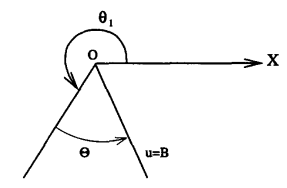
\includegraphics[scale=0.5]{Images/rotated_wedge.png}
        \caption{Rotation of the wedge domain. Image taken from \cite{li2000singularities}.}
        \label{rotated_wedge}
    \end{figure}
    In applications, we are mostly concerned with Dirichlet-Neumann and Neumann-Dirichlet boundary conditions. Just like stated above, some of these boundary conditions have different expansions for the angles \(\Theta=\frac{\pi}{2}\) and \(\Theta=\frac{3\pi}{2}\). However, we are only concerned with the expansion
    \[
        v(r,\theta) = \sum_{k=0}^{\infty}\alpha_k r^{\alpha_k}\psi(\alpha_k \theta)
    \]
    where \(\psi=\sin\) or \(\psi = \cos\). In these cases, if we neglect the other terms, for the special angle \(\Theta = \frac{\pi}{2}\) above we would find that \(\alpha_k \in \mathbb{N}\). Without going into much dept in singularity analysis, then its partial derivative \(\partial_r v(r,\theta)\) would be of the form 
    \[
        \partial_r v(r,\theta) = \sum_{k=0}^{\infty}\alpha_k^2 r^{\alpha_k-1}\psi(\alpha_k \theta)
    \]
    where \(\alpha_k-1 \in \mathbb{N}\). In general, if \(\alpha_k \in \mathbb{N}\) for some angle \(\Theta\) then all of its derivatives are continuous and \(v(r,\theta)\) is analytical. More precisely, there is no singularity in these cases. Therefore, one does not need to enrich the set of basis functions since the fundamental solutions correctly reproduce the behavior near the corner's tip. Such corners are called \textit{regular}. On the other hand, corners that present singularities are called \textit{singular} and are the ones that we are interested to approximate. 

    Also notice that, in the expansions above, the term \(r^{-\alpha_k}\) does not appear. This has to do with the fact we are dealing with an interior problem: when considering the exterior problem, the terms \(r^{\alpha_k}\) are replaced with \(r^{-\alpha_k}\) (observe that it satisfies the asymptotic conditions prescribed in order to have well-posedness of the exterior problem!).
\end{remark}

\section{The Subspace Angle Technique} \label{sat_appendix}

One of the drawbacks of the \ac{MFS} is the ill-conditioning of the system. In this subsection we introduce the so-called \textit{Subspace Angle Technique}, first presented in \cite{betcke2005reviving}. Intuitively, there are two problems at play: firstly, while the \ac{MFS} only needs the boundary data to approximate the solution of the \ac{BVP}, the exponential growth of the condition number against its exponential convergence can be seen has the lack of information given by the collocation points on the boundary, which is not enough to decide if an approximate eigenfunction is spurious; secondly, while we proved the linear independence of the basis functions, in practice the columns of the matrix \(A(k)\) are almost linear dependent if its number is too large (in fact, this is, once again, associated with the distance from the boundary to the artificial boundary).

To solve the first problem, we add additional interior points in order to over-determine the system; and for the second problem, we construct an orthonormal basis of the column space of \(A(k)\), denoted by \(\mathcal{C}(A(k))\), using the \(QR\) factorization of \(A(k)\). Let \(M_B\) be the number of boundary points and \(M_I\) the number of interior points, such that \(M=M_B+M_I\). Then, by adding some interior points the matrix \(A(k)\) can be extended to
\[
    A(k) = \begin{bmatrix}
        A_B(k)\\
        A_I(k)
    \end{bmatrix},
\]
where the indices \(B\) and \(I\) correspond to the block matrices with the boundary and interior collocation points, respectively. To generate an orthonormal basis of the column space of \(A(k)\), consider the \(QR\) factorization of \(A(k)\), given by \(A(k)=Q(k)R\), where \(Q(k)\) is a unitary complex (possible non-rectangular) matrix. By partitioning \(Q(k)\) in the boundary and interior collocation points, we also have
\begin{equation*}
    Q(k) = \begin{bmatrix}
        Q_B(k)\\
        Q_I(k)
    \end{bmatrix},
\end{equation*}
and each unit vector \(u \in \mathcal{C}(A(k))\) has the form
\begin{equation}\label{sat_qr}
    u = \begin{bmatrix}
        u_B\\
        u_I
    \end{bmatrix} = Q(k)v = \begin{bmatrix}
        Q_B(k)\\
        Q_I(k)
    \end{bmatrix}v
\end{equation}
for some \(v \in \mathbb{R}^2\), \(\norm*{v} = 1\). Assuming homogeneous Dirichlet boundary conditions, we are interested in non-trivial solutions \(v \in \mathbb{R}^2\) to the above problem when \(u \approx 0\) at the boundary, i.e., to solve the constrained minimization problem
\[
    \min_{v \in \mathbb{R}^2, \norm*{v}=1} \norm*{Q_B(k) v}. 
\]
The above problem is easy to solve and has a closed-form solution which can be found using Lagrange multipliers. The solution \(\check{v}\) is the right singular vector of \(Q_B(k)\) associated with the smallest singular value \(\sigma_N\) and
\[
    \sigma_N(k) = \norm*{Q_B(k) \check{v}}.
\]
Let \(\check{u} = Q(k) \check{v}\). By taking the norm on both sides of equation \eqref{sat_qr}, one can write
\begin{equation}\label{sat_eq}
    1 = \norm{\check{u}}^2 = \norm{\begin{bmatrix}
        Q_B(k)\\
        Q_I(k)
    \end{bmatrix}\check{v}}^2 = \sigma_N^2(k) + \norm*{Q_I(k) \check{v}}^2.
\end{equation}
Notice how equation \eqref{sat_eq} can be used to eliminate spurious solutions: since \(0 < \sigma_N < 1\), if \(\sigma_N \approx 1\), then \(Q_I(k) \check{v} \approx 0 \implies u_I \approx 0\) which is an incorrect solution (is zero on the interior and does not satisfy the boundary constraints); on the other hand, if \(\sigma_N \approx 0\), then we found an eigenfunction which is small on the boundary points and whose interior is not null.

The name Subspace Angle Technique comes from the fact that \(\sigma_N\) is related to the angle between the subspaces \(\mathcal{C}(A(k))\) and \(\mathcal{G}_0\), the space of vectors that are zero at boundary points\footnote{\(\mathcal{G}_0\) can be seen as the discretization of the functions which satisfy the boundary conditions but not the Helmholtz equation.}. The angle \(\phi(k)=\angle (\mathcal{C}(A(k)), \mathcal{G}_0)\) between both subspaces is defined by
\[
    \cos \phi(k) = \sup_{\substack{u \in \mathcal{C}(A(k)), \, \norm{u}=1 \\ v \in \mathcal{G}_0, \, \norm*{v} = 1}} (u, v),
\]
and one can prove (cf. \cite{betcke2005reviving}) that
\[
    \sigma_N = \sin \phi(k).
\]
Therefore, the discrete problem has a non-trivial solution (i.e., \(\lambda\) is an eigenvalue of the Laplace operator) if and only if \(\mathcal{C}(A(k))\) and \(\mathcal{G}_0\) have a non-trivial intersection (i.e., \(\phi(k) = l \pi, \, l \in \mathbb{Z}\)).

\begin{remark}
    While the construction above assumed homogeneous Dirichlet boundary conditions, it can be easily generalized to any type of homogeneous boundary conditions \(\mathcal{B}\) by considering the appropriate \(A\) matrix.
\end{remark}

\begin{remark}
    Neither the enrichment technique with particular solutions nor the Subspace Angle Technique are specific methods only applicable to the Laplace equation and the Helmholtz equation, respectively. They can be used for both equations at the same time. For example, in \cite{antunes2010meshfree}, both methods were used to study the spectrum of the Laplace operator in domains with corners and cracks.
\end{remark}